\hypertarget{limits-of-casual-loop-diagrams}{%
\section{Limits of casual loop
diagrams}\label{limits-of-casual-loop-diagrams}}

\begin{figure}
\centering
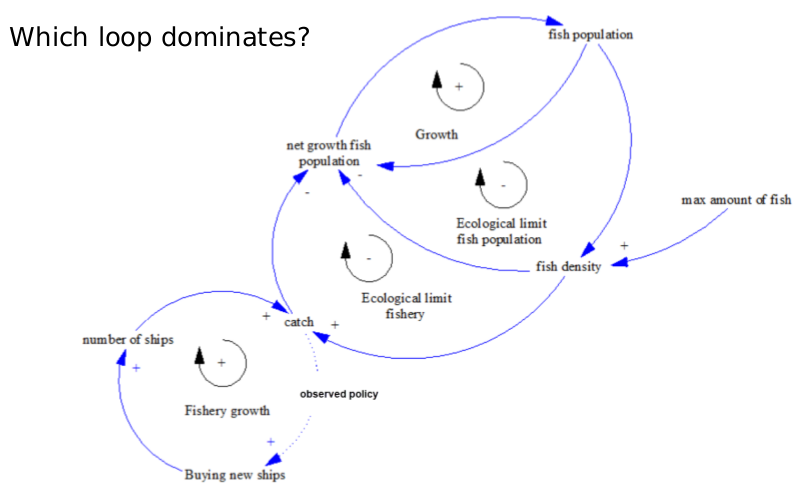
\includegraphics{figures/limitsCld.png}
\caption{Limits of CLDs}
\end{figure}

\hypertarget{domination}{%
\subsection{1. Domination}\label{domination}}

With CLDs only and no simulation model, it is not possible to determine
which loop dominates.

\hypertarget{collapse-point-of-a-system}{%
\subsection{2. Collapse point of a
system}\label{collapse-point-of-a-system}}

Saturation points are not modelled. Like when are enough fish in the
sea.

\hypertarget{loop-interaction}{%
\subsection{3. Loop interaction}\label{loop-interaction}}

On basis of the CLD it is not possible to figure out, how the loops will
interact. The importance of the loops are not modelled.

\hypertarget{fundamental-modes-of-dynamic-behavior}{%
\section{Fundamental modes of dynamic
behavior}\label{fundamental-modes-of-dynamic-behavior}}

\begin{figure}
\centering
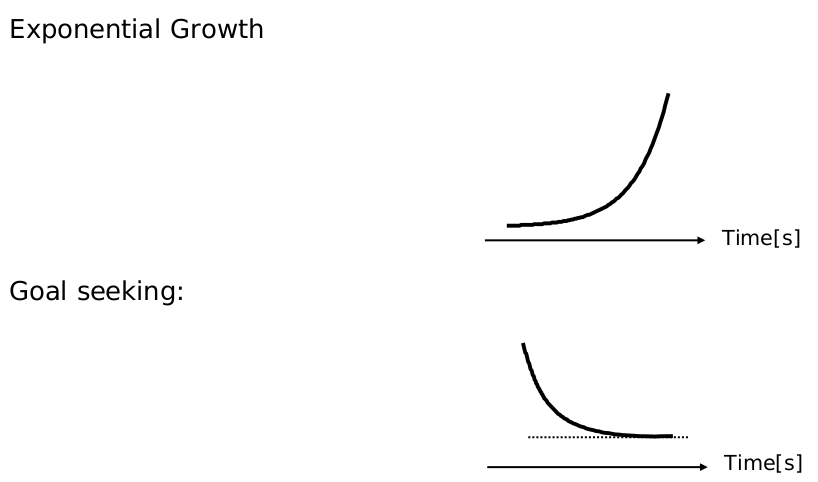
\includegraphics{figures/fundamentalModesDynamicBehavior1.png}
\caption{Fundamental modes of Dynamic Behaviors 1}
\end{figure}

\begin{figure}
\centering
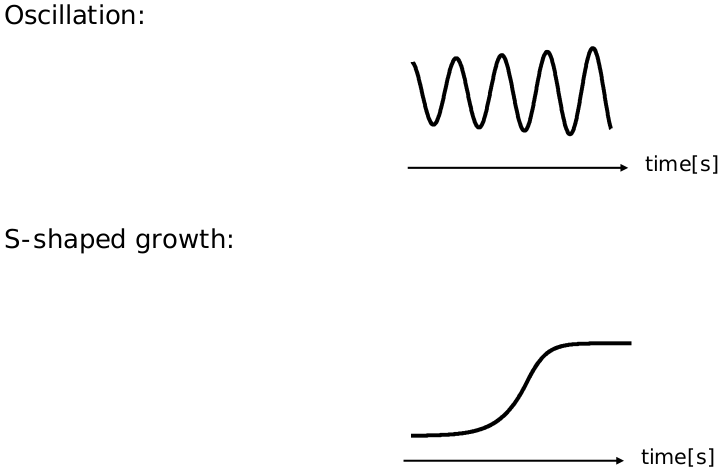
\includegraphics{figures/fundamentalModesDynamicBehavior2.png}
\caption{Fundamental modes of Dynamic Behaviors 2}
\end{figure}

\begin{figure}
\centering
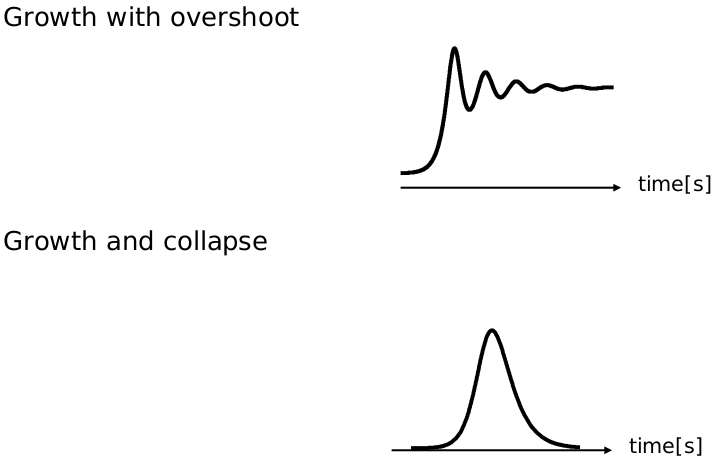
\includegraphics{figures/fundamentalModesDynamicBehavior3.png}
\caption{Fundamental modes of Dynamic Behaviors 3}
\end{figure}

\hypertarget{the-matter-of-time}{%
\subsection{The matter of time}\label{the-matter-of-time}}

\begin{figure}
\centering
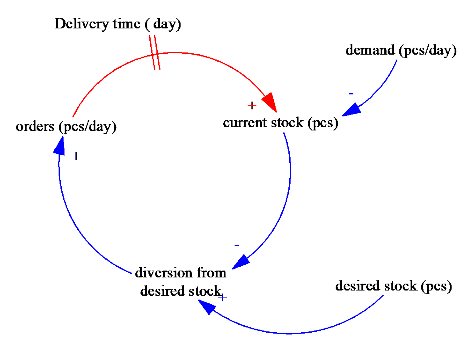
\includegraphics{figures/oscillationDelay.png}
\caption{Oscillation}
\end{figure}
